\section{Evolution of dark solitons in a homogeneous 1D Bose gas}

We start our analysis by initializing the density distribution on a spatial grid of length $L = 240$ with $2048$ grid points, containing $2048$ particles.

We took to analytic solution from equation (\ref{eqn:analytic}) at $t=0$ and used our implementation of the Split-Step Fourier method to determine its evolution, using a step size of $\dd t = 0.01$. In total, we computed $N_{\text{steps}} = 800$ time steps. To discuss the results, we included some pictures of different time steps in the following. The animated evolution can be found in the corresponding Python notebook.

\subsection{Single black soliton}
We initialize a black soliton at $z_0 = 0$.
 \begin{figure}[H]
 \centering
 \begin{subfigure}{0.42\textwidth} 
 	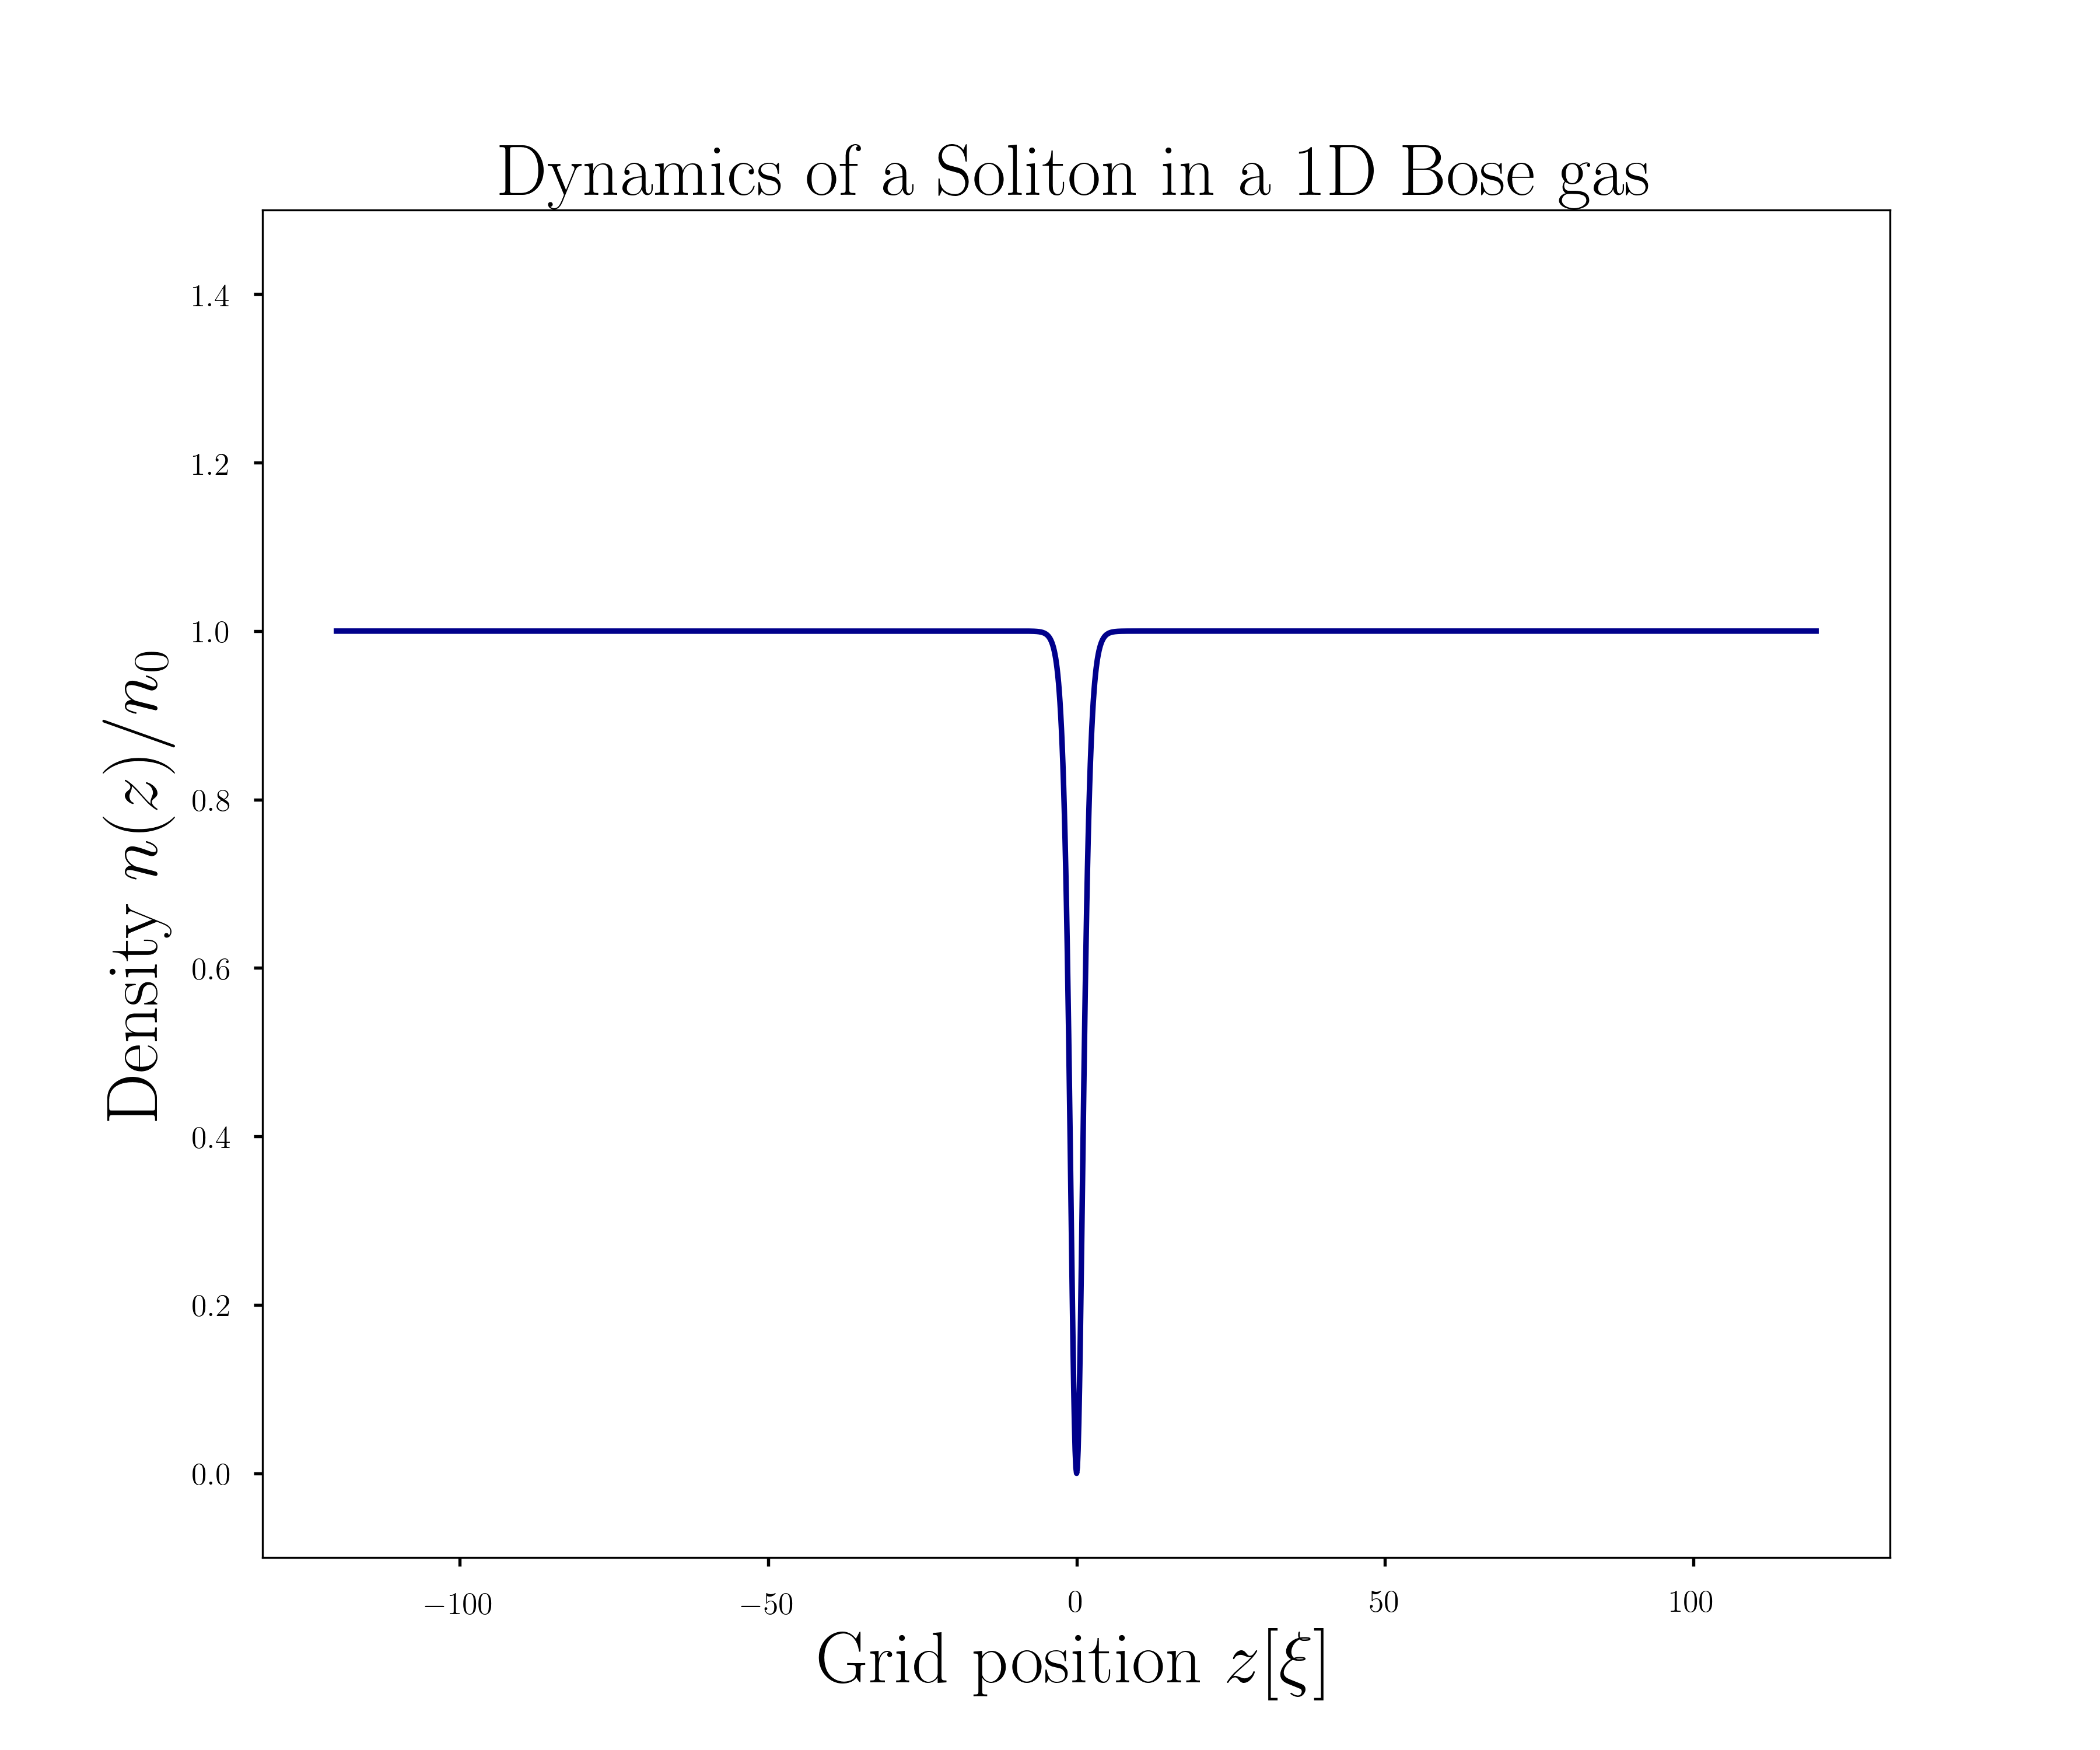
\includegraphics[width= \textwidth]{figures/single_black_0}
 	\subcaption{Initial state}
 \end{subfigure}
 \begin{subfigure}{0.42\textwidth} 
 	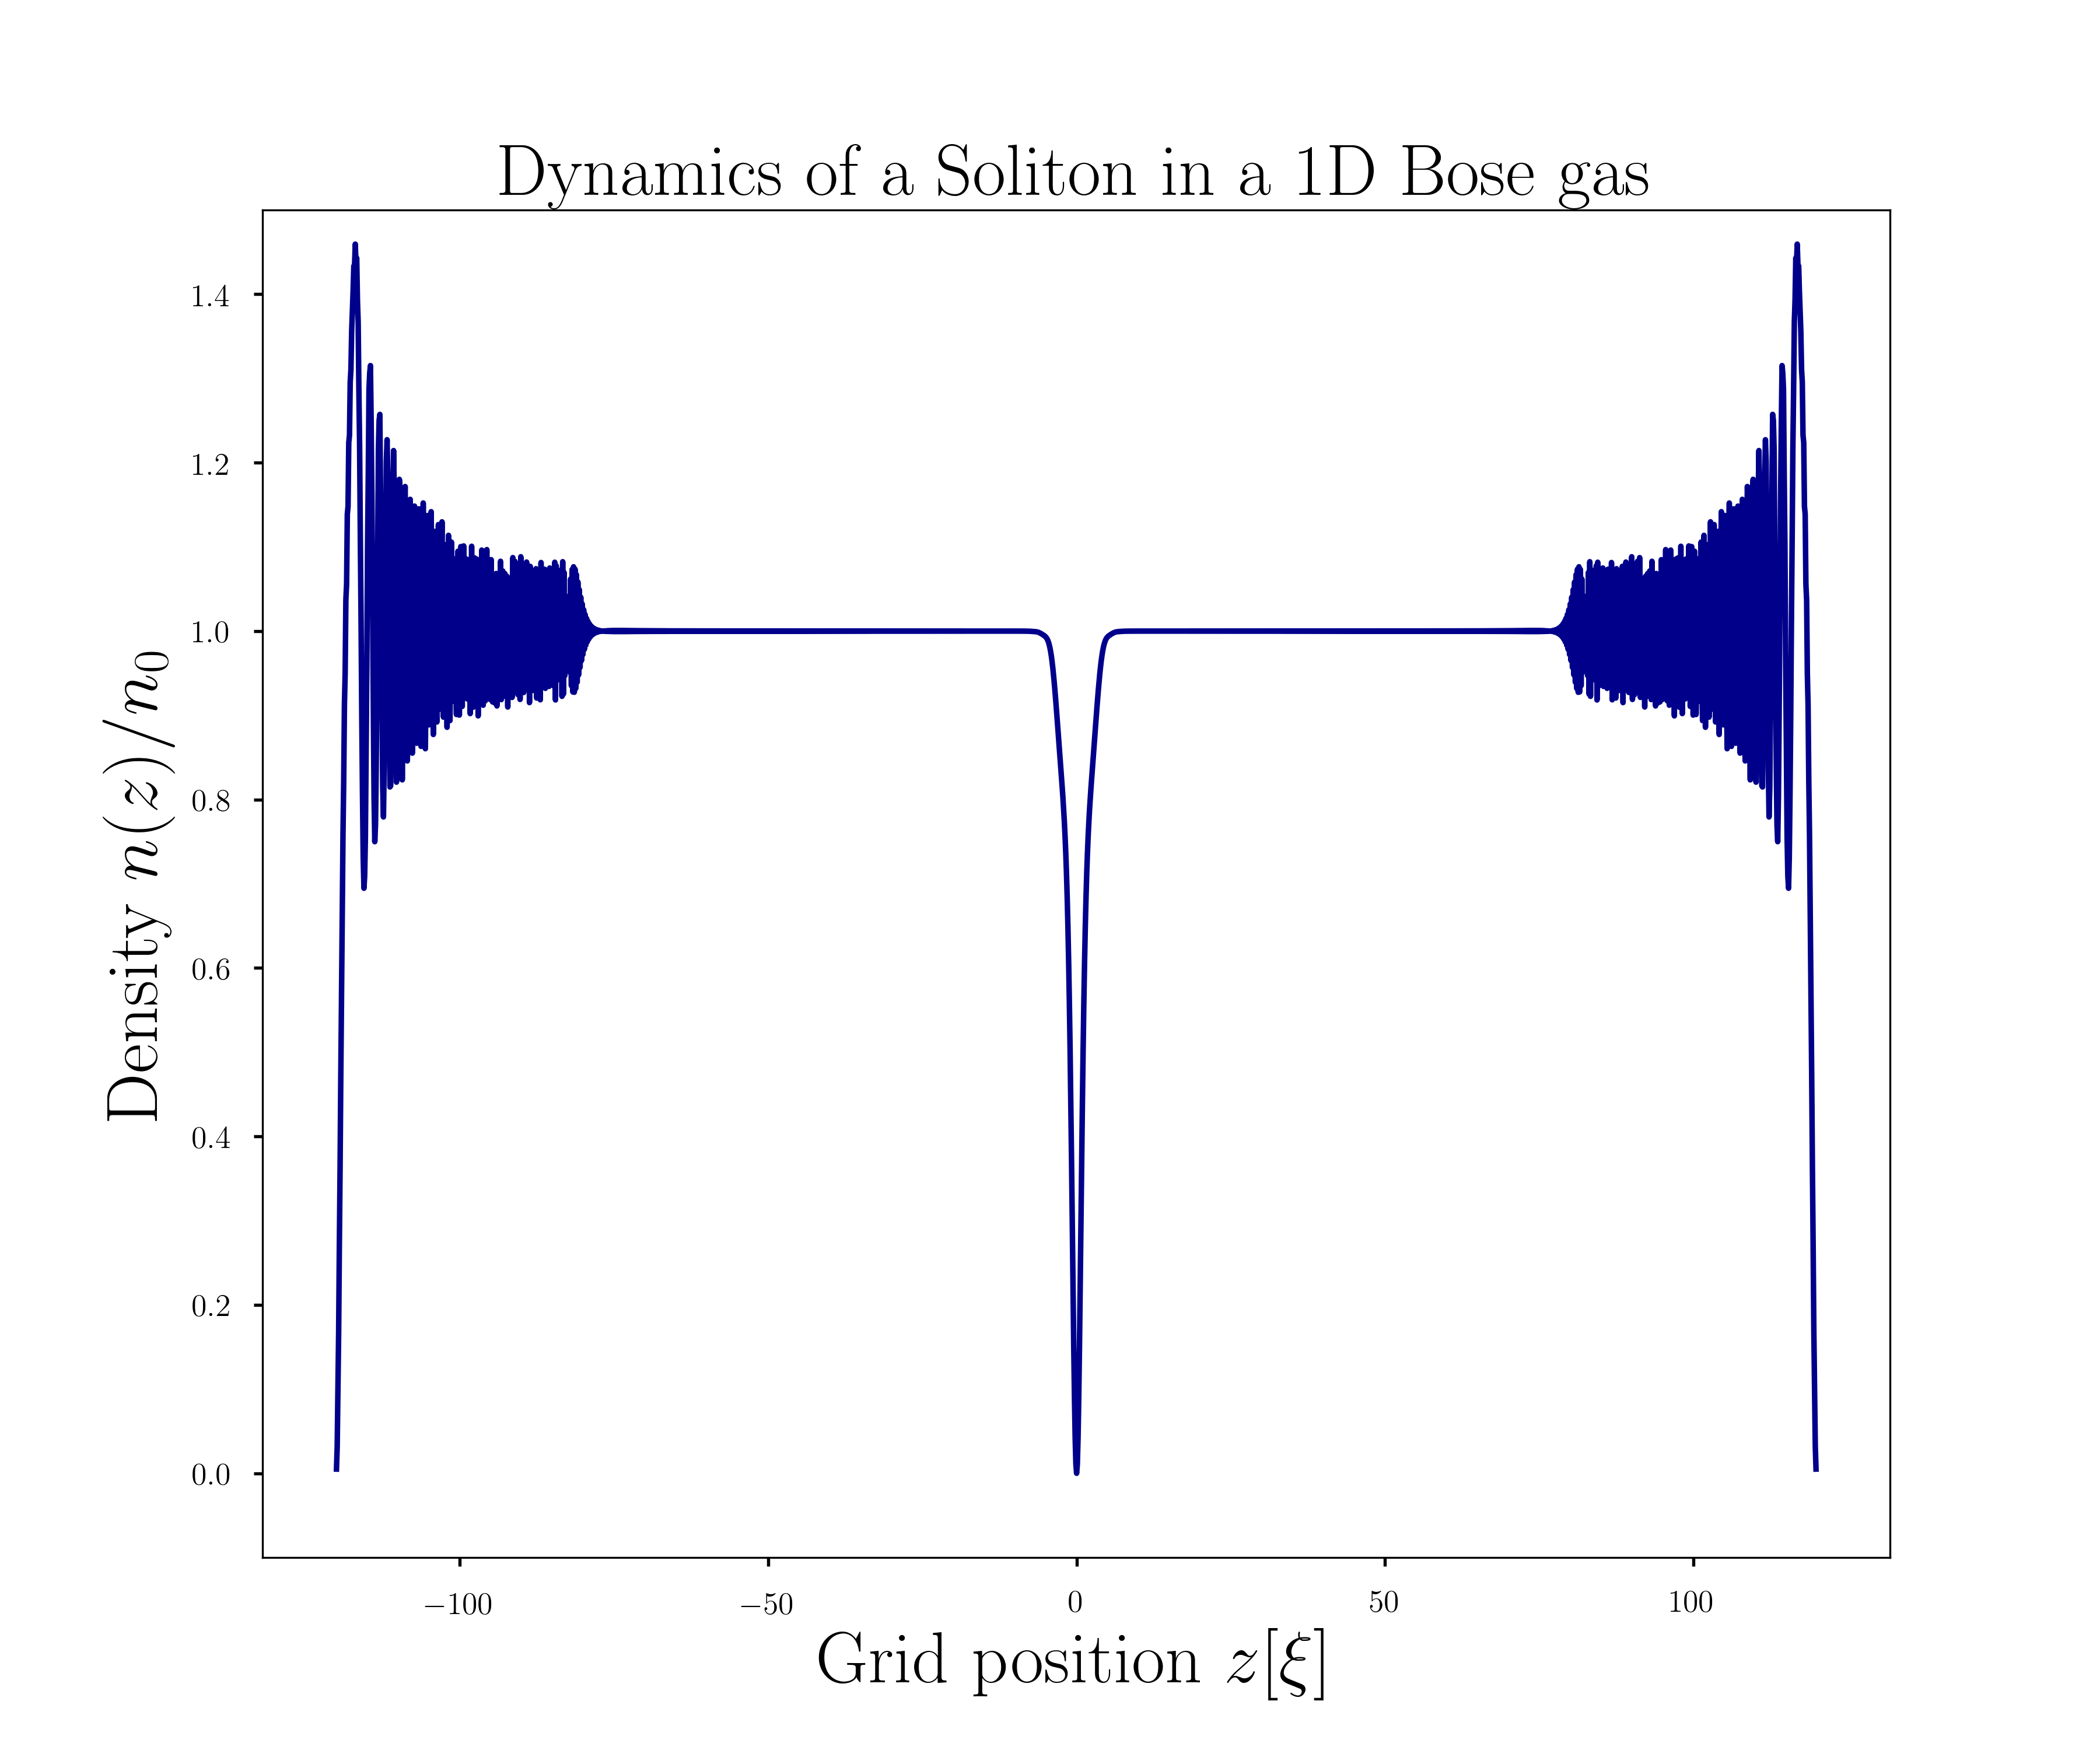
\includegraphics[width= \textwidth]{figures/single_black_150}
 	\subcaption{After $N_{\text{steps}} = 150$.}
 \end{subfigure}
 \caption{Dynamics of a single black soliton}	
 \end{figure}
 \newpage
\subsection{Single grey soliton}
We initialize a soliton with greyness $\nu = 0.8$ at $z_0 = 0$.
 \begin{figure}[H]
 \centering
 \begin{subfigure}{0.42\textwidth} 
 	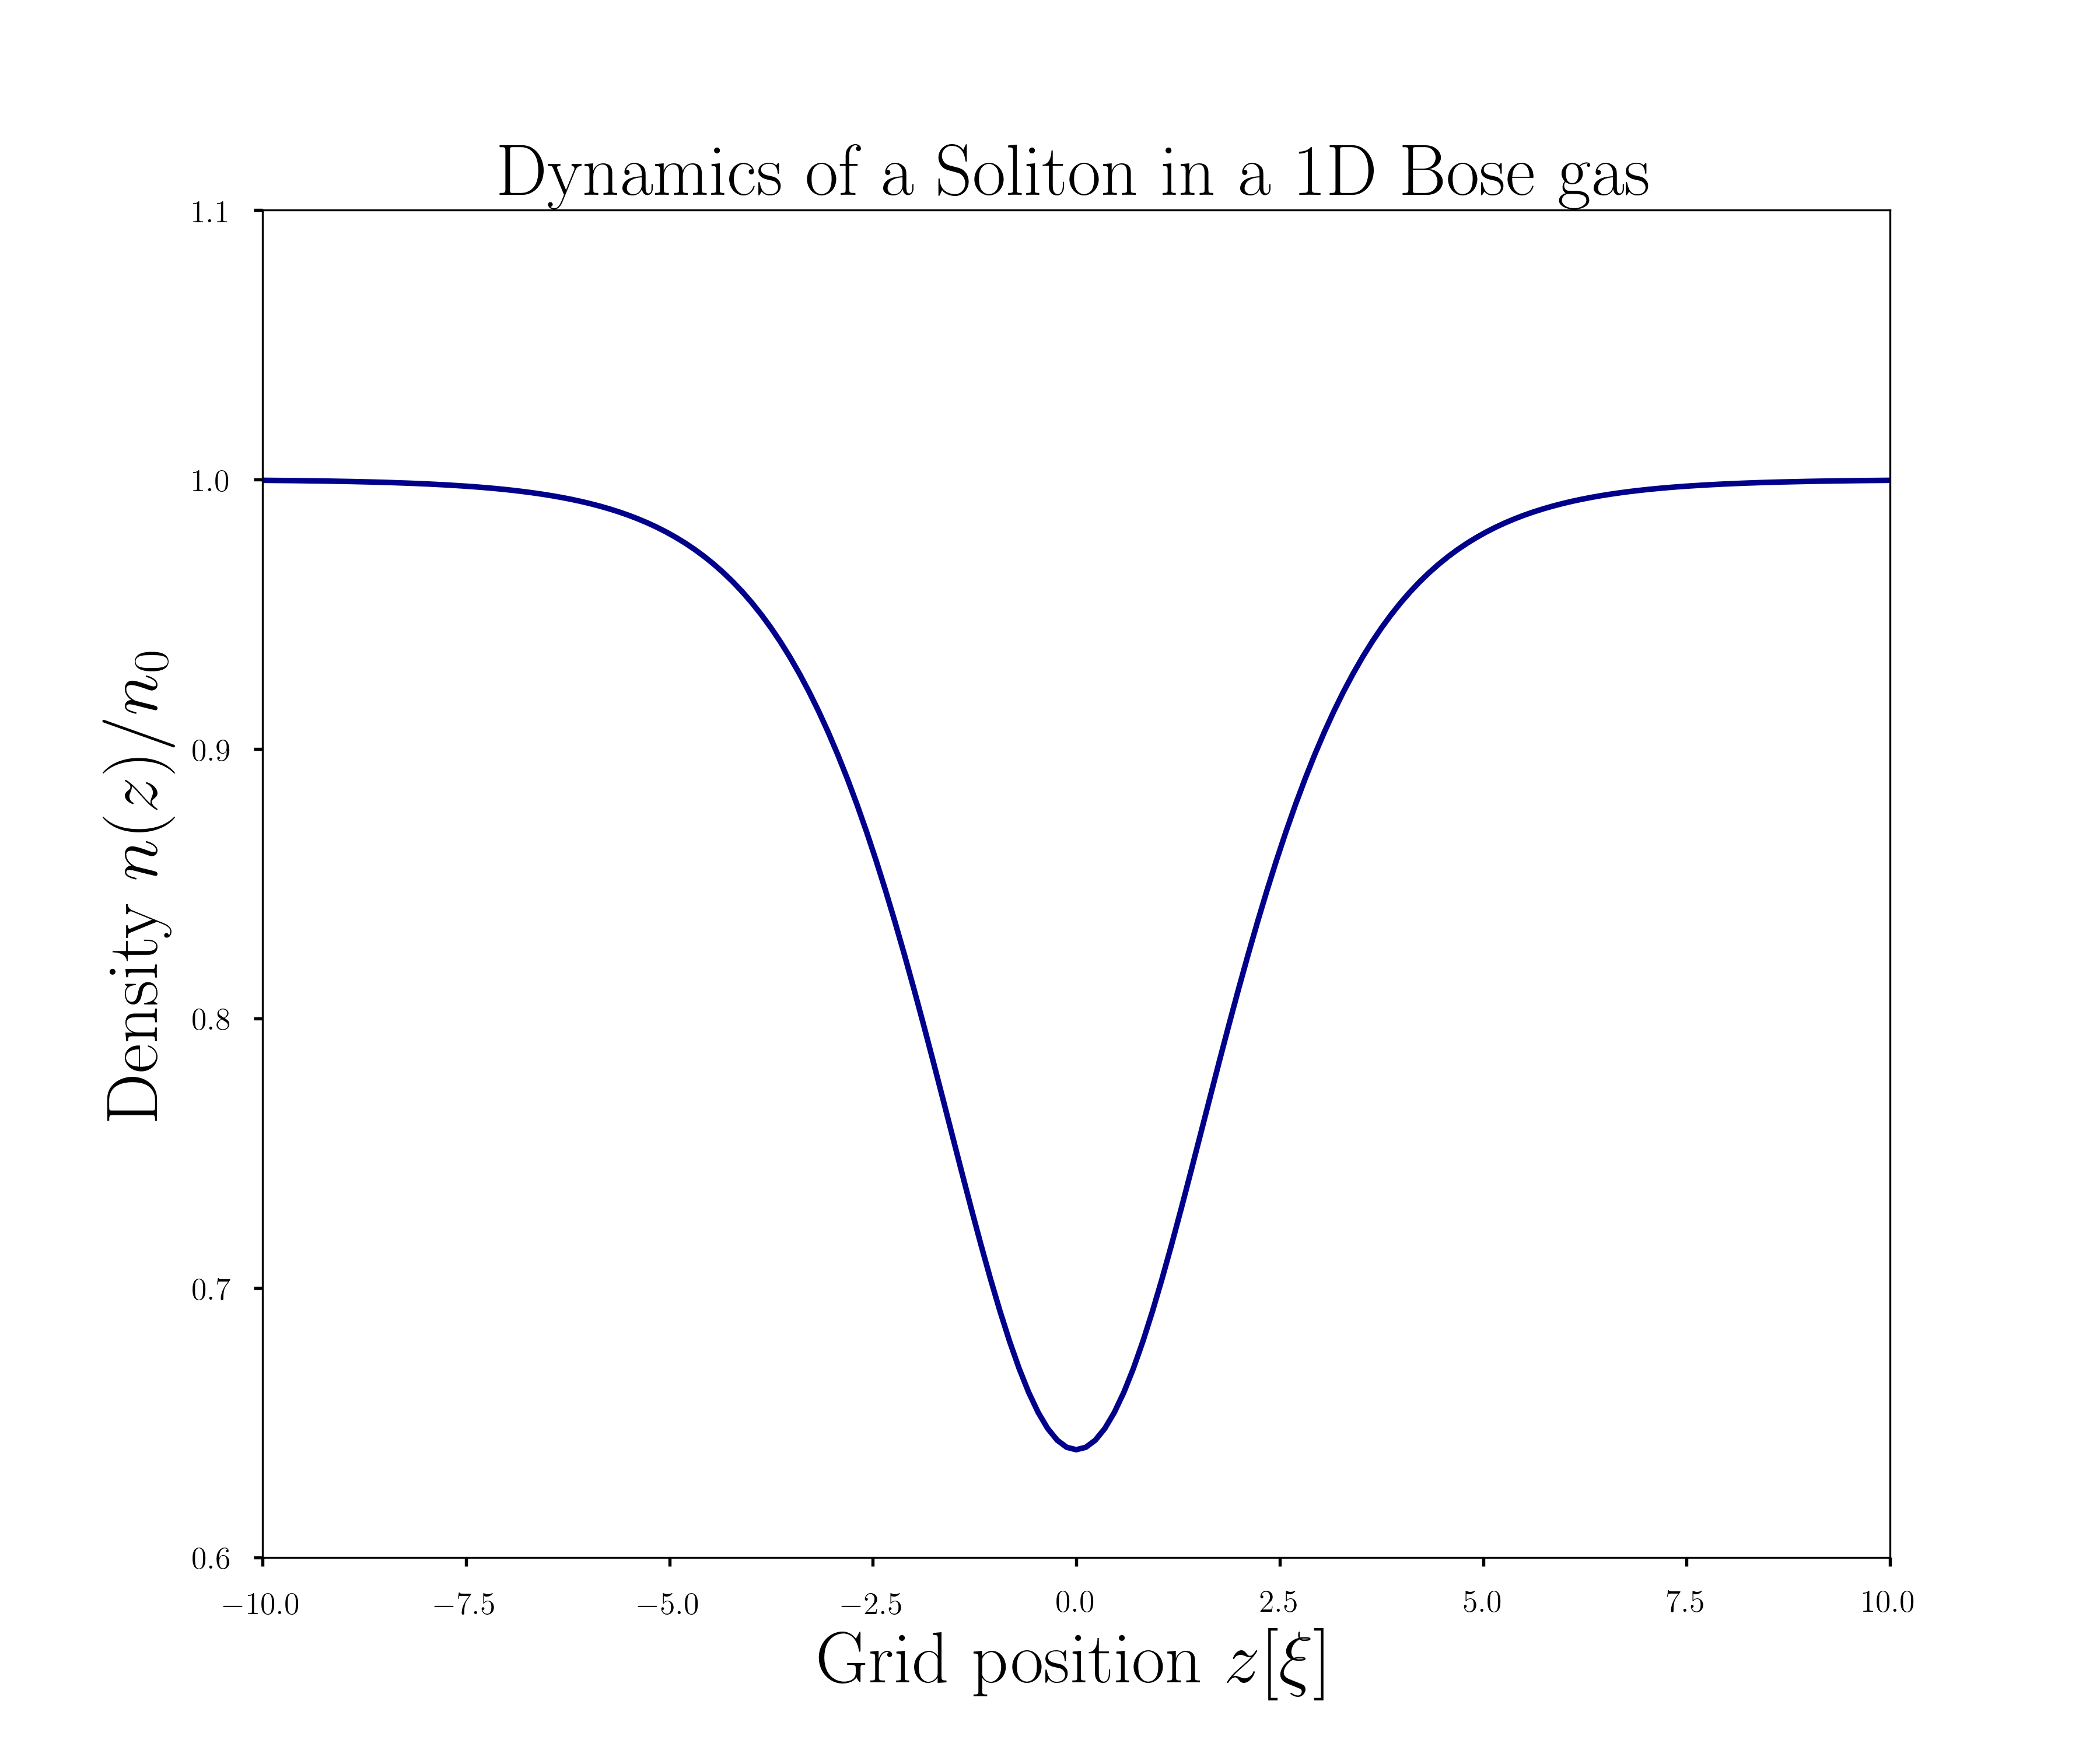
\includegraphics[width= \textwidth]{figures/single_grey_0}
 	\subcaption{Initial state}
 \end{subfigure}
 \begin{subfigure}{0.42\textwidth} 
 	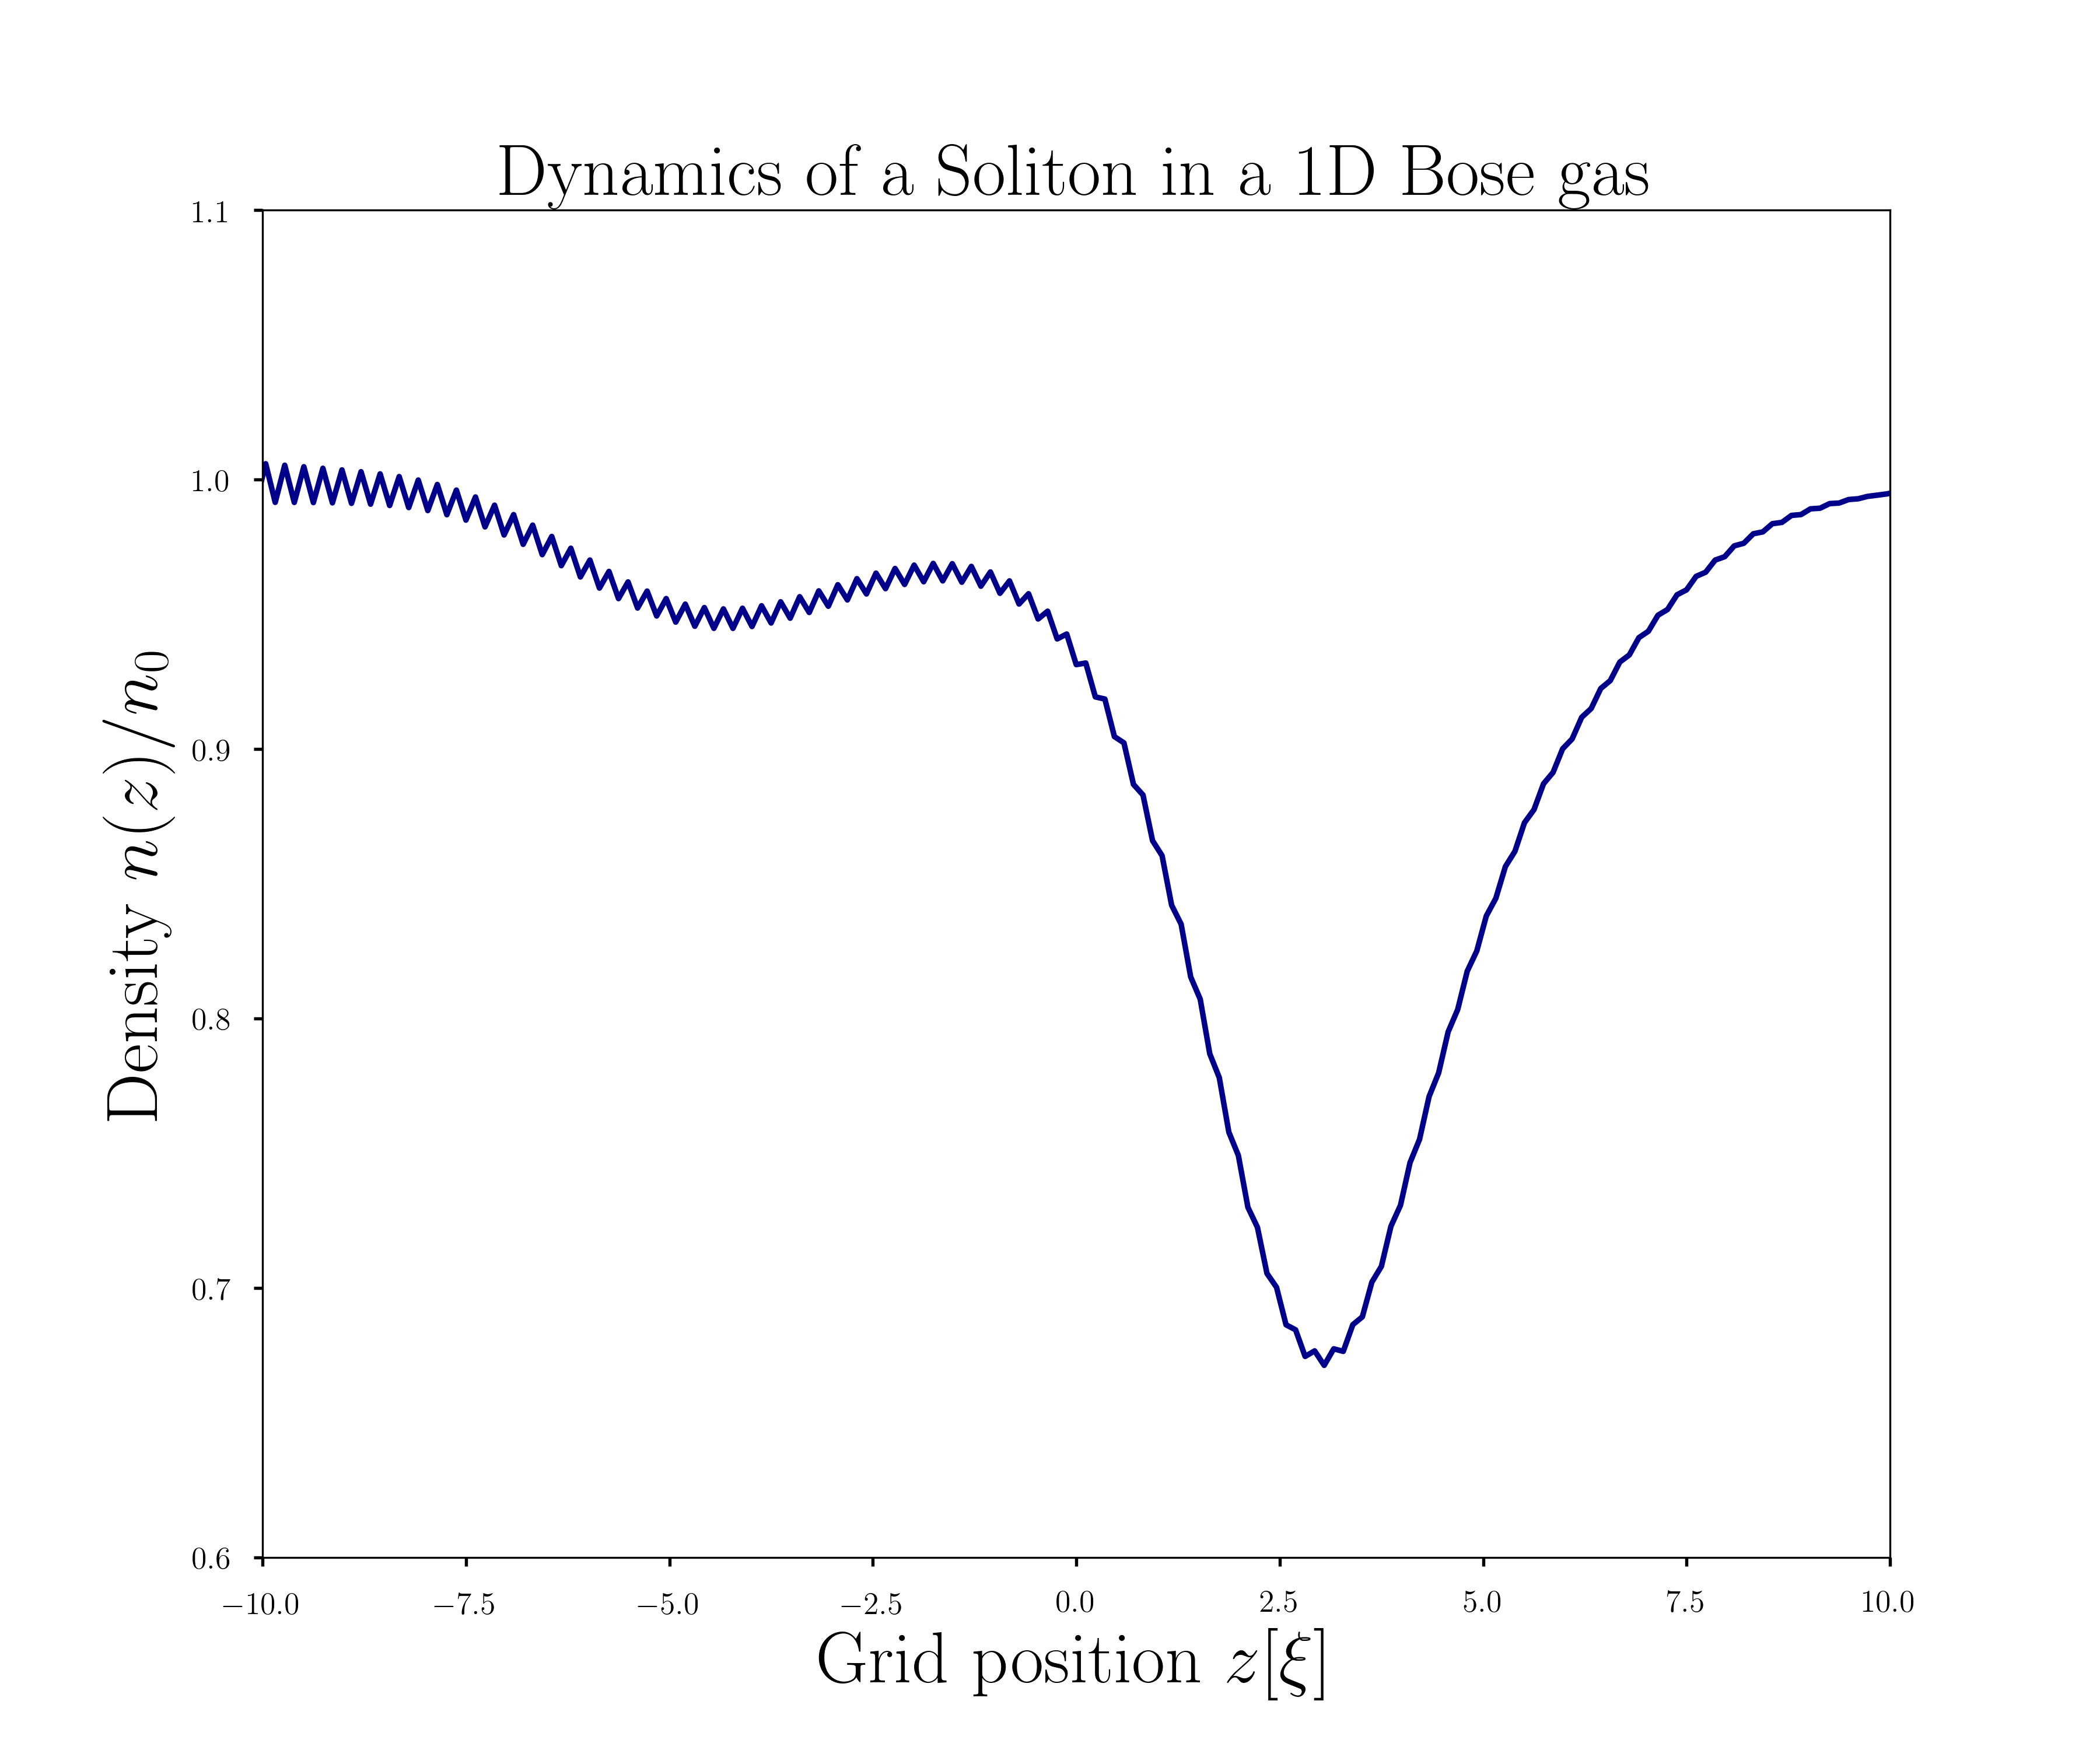
\includegraphics[width= \textwidth]{figures/single_grey_400}
 	\subcaption{After $N_{\text{steps}} = 400$.}
 \end{subfigure}
 \caption{Dynamics of a single grey soliton}	
 \end{figure}
 
\subsection{Two grey solitons moving in opposite directions}
We initialize two solitons with greyness $\nu_1 = \nu_2 = 0.8$ at $z_{1,2} = \pm \ 3.5$.
 \begin{figure}[H]
 \centering
  \begin{subfigure}{0.42\textwidth} 
 	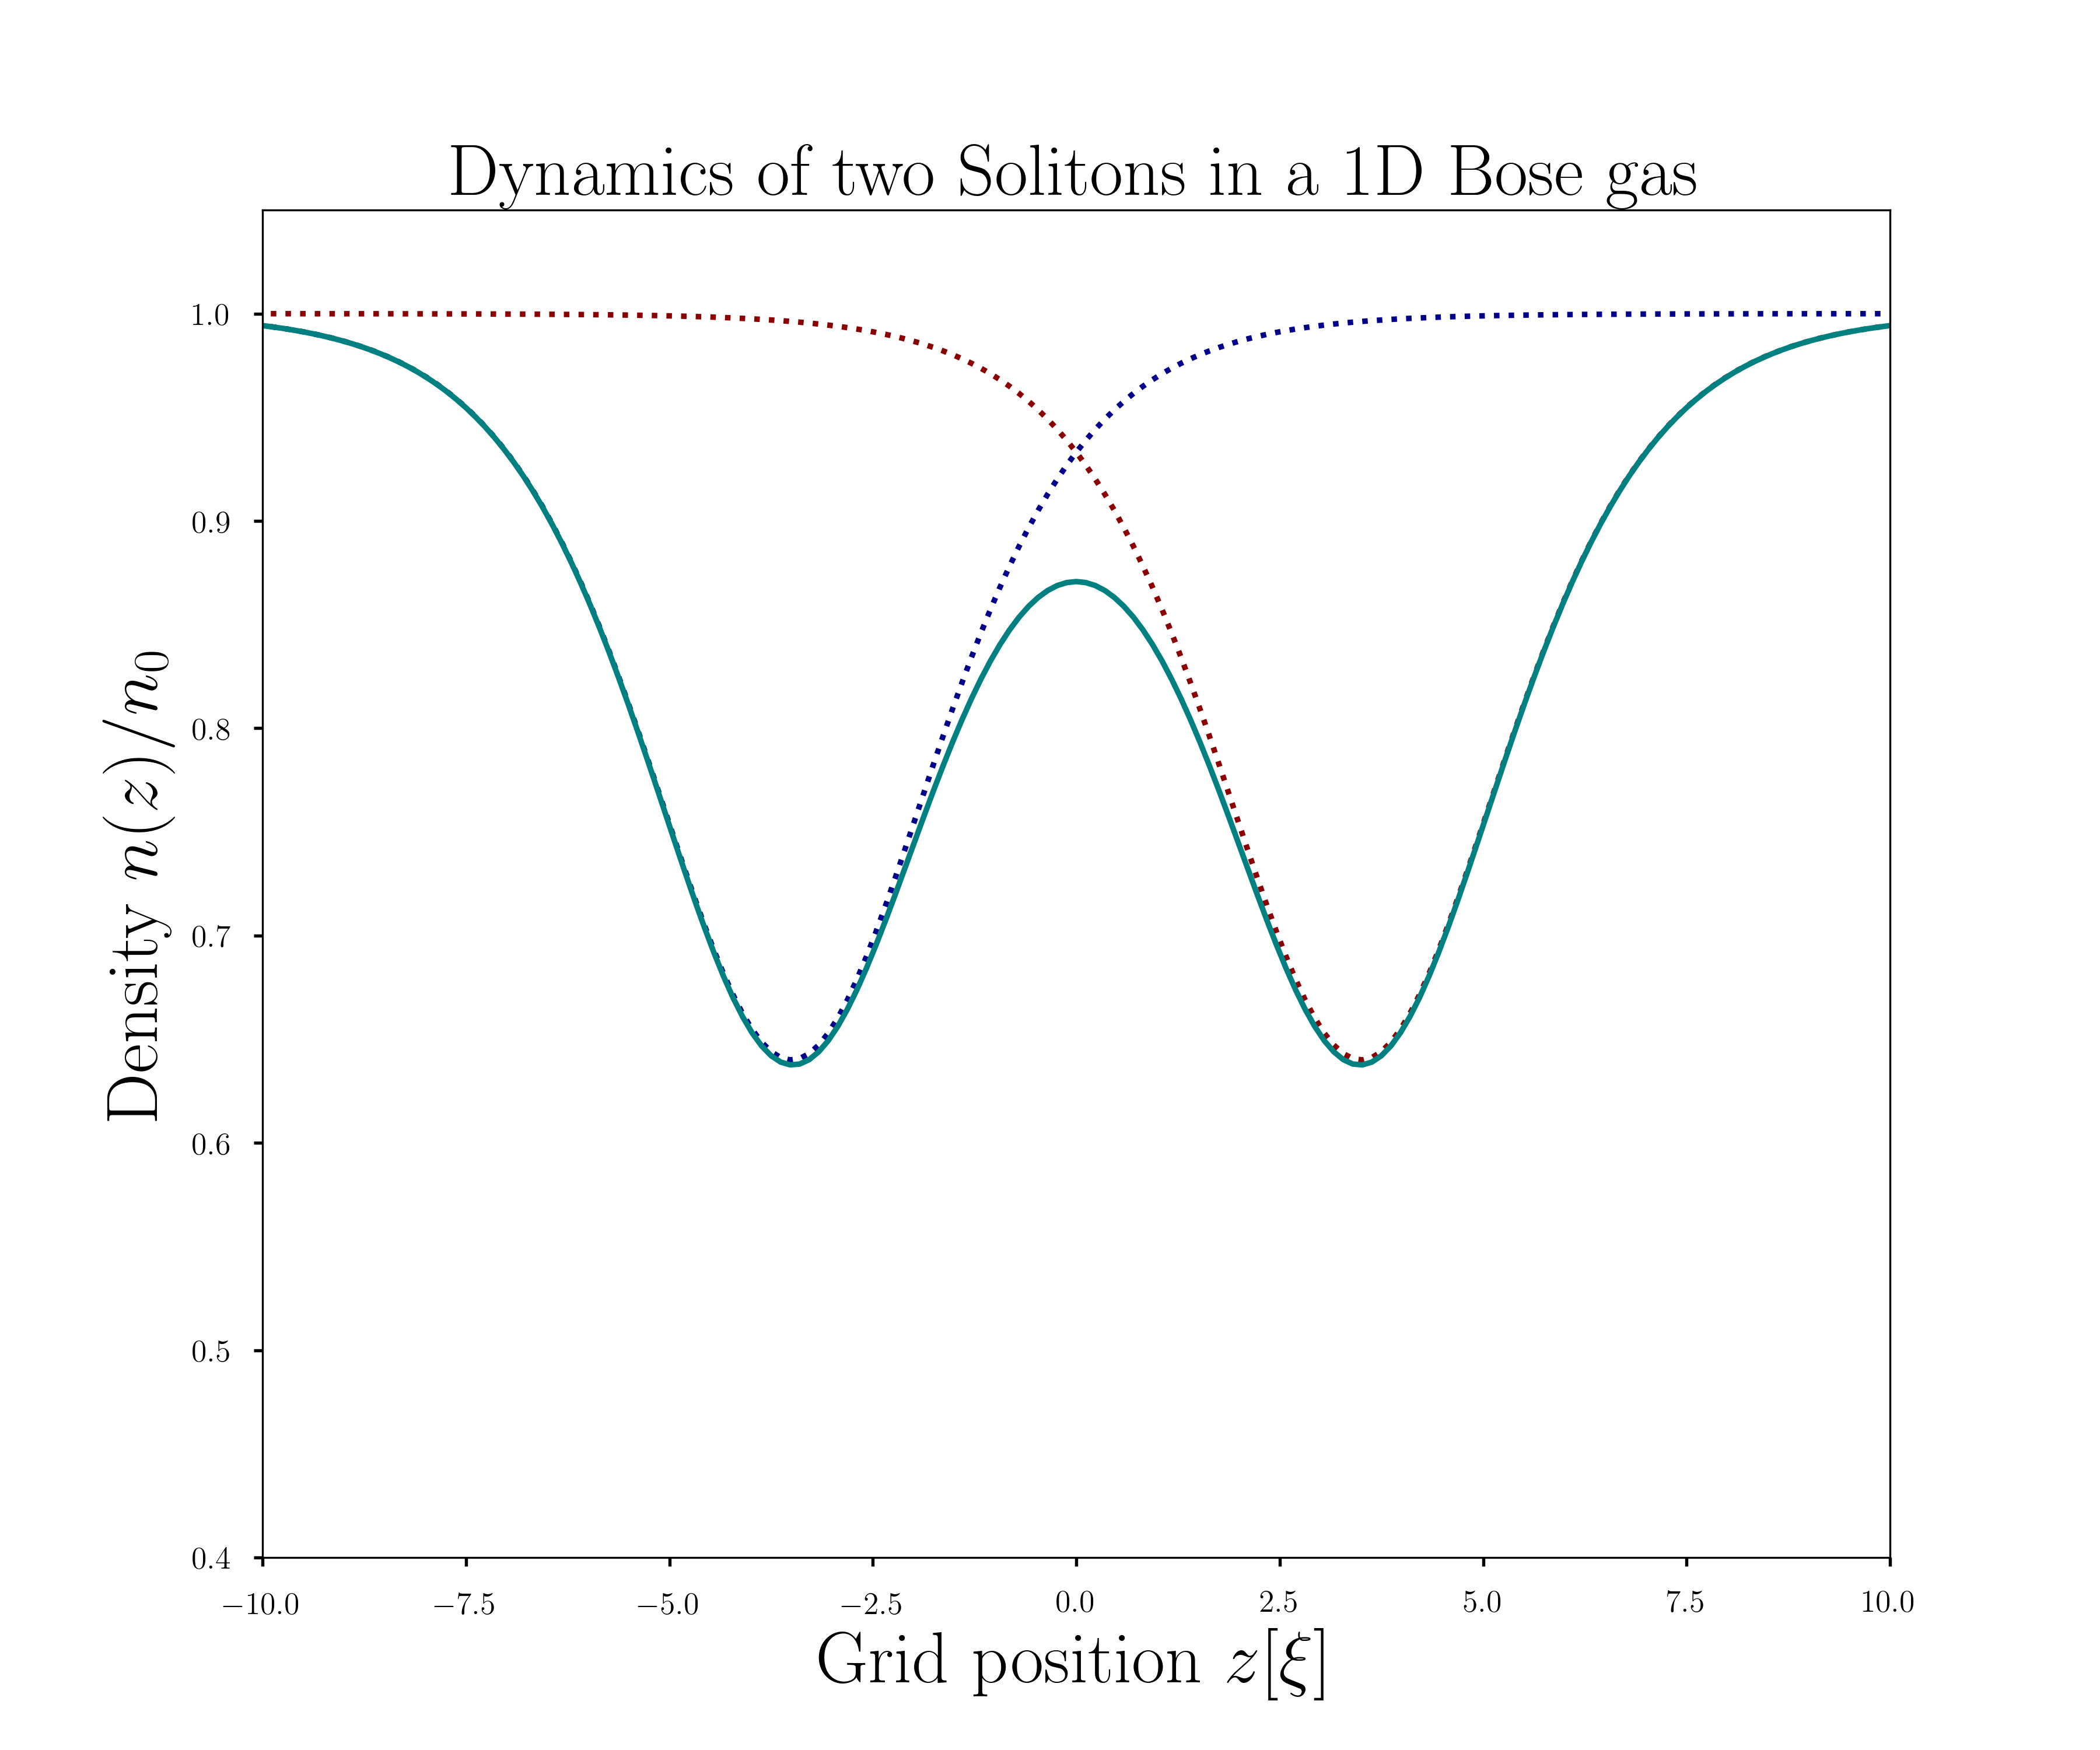
\includegraphics[width= \textwidth]{figures/two_grey_3_5_0}
 	\subcaption{Initial state}
 \end{subfigure}
 \begin{subfigure}{0.42\textwidth} 
 	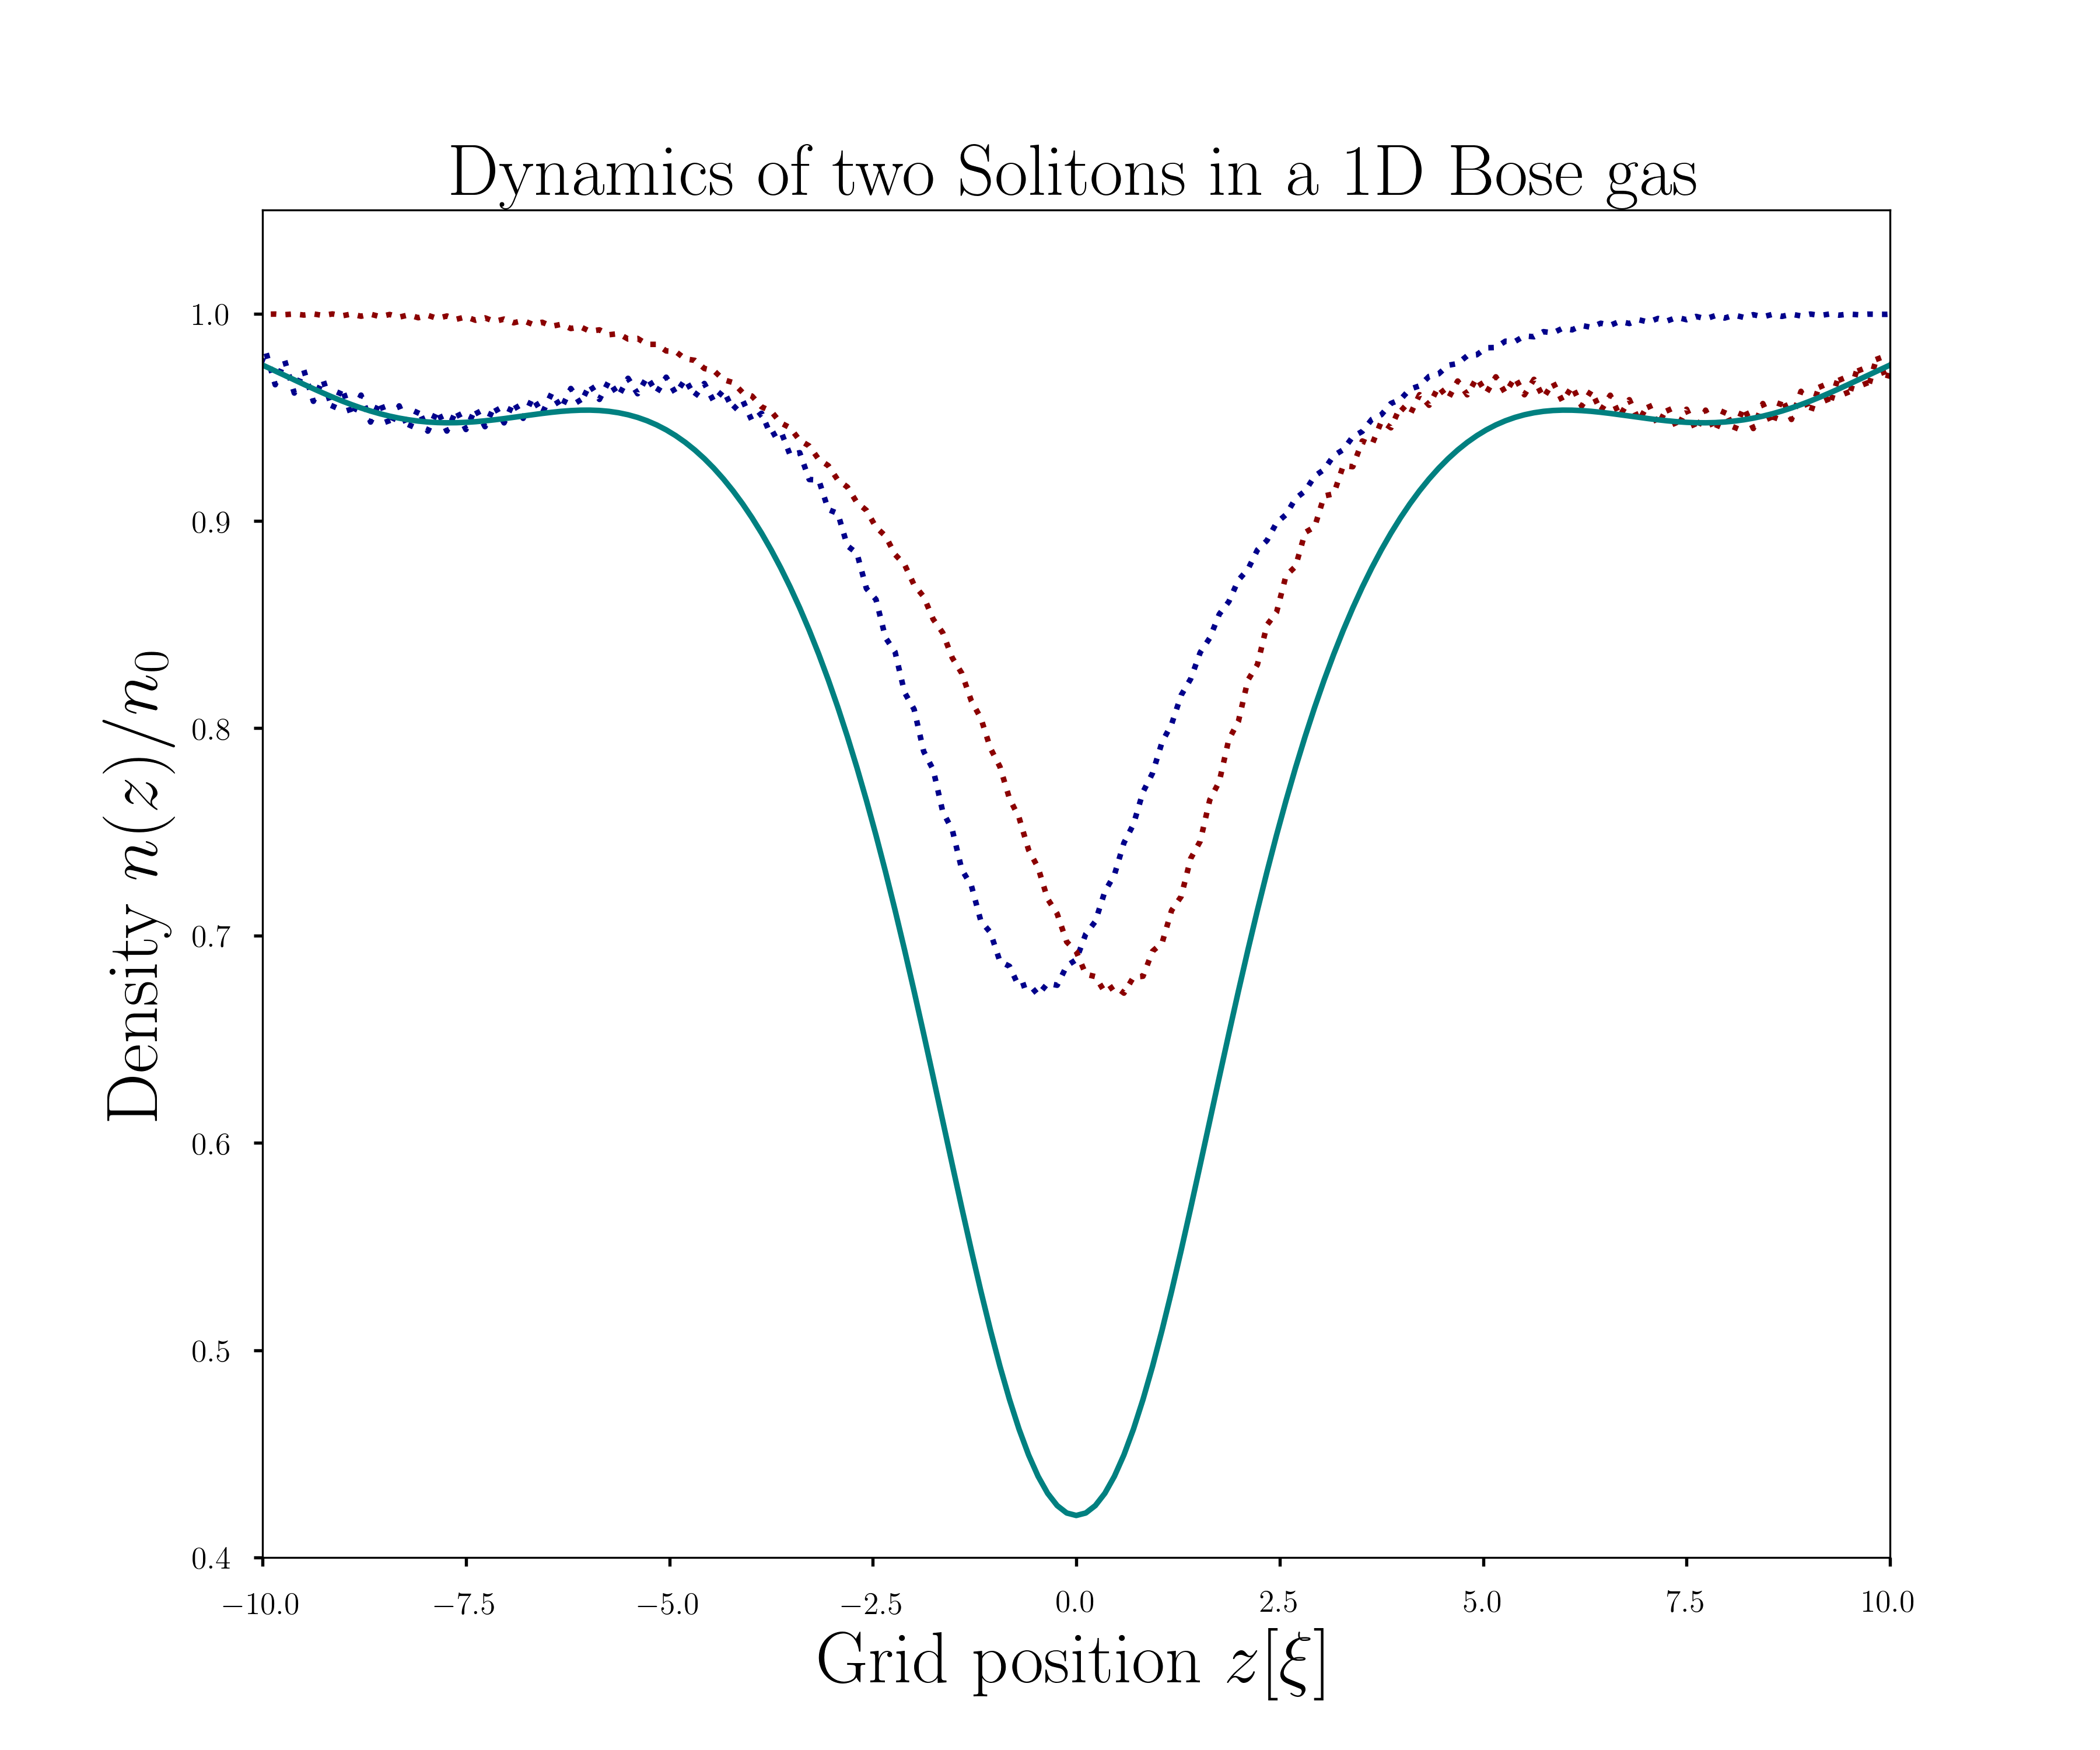
\includegraphics[width= \textwidth]{figures/two_grey_3_5_400}
 	\subcaption{After $N_{\text{steps}} = 400$.}
 \end{subfigure}
 \begin{subfigure}{0.42\textwidth} 
 	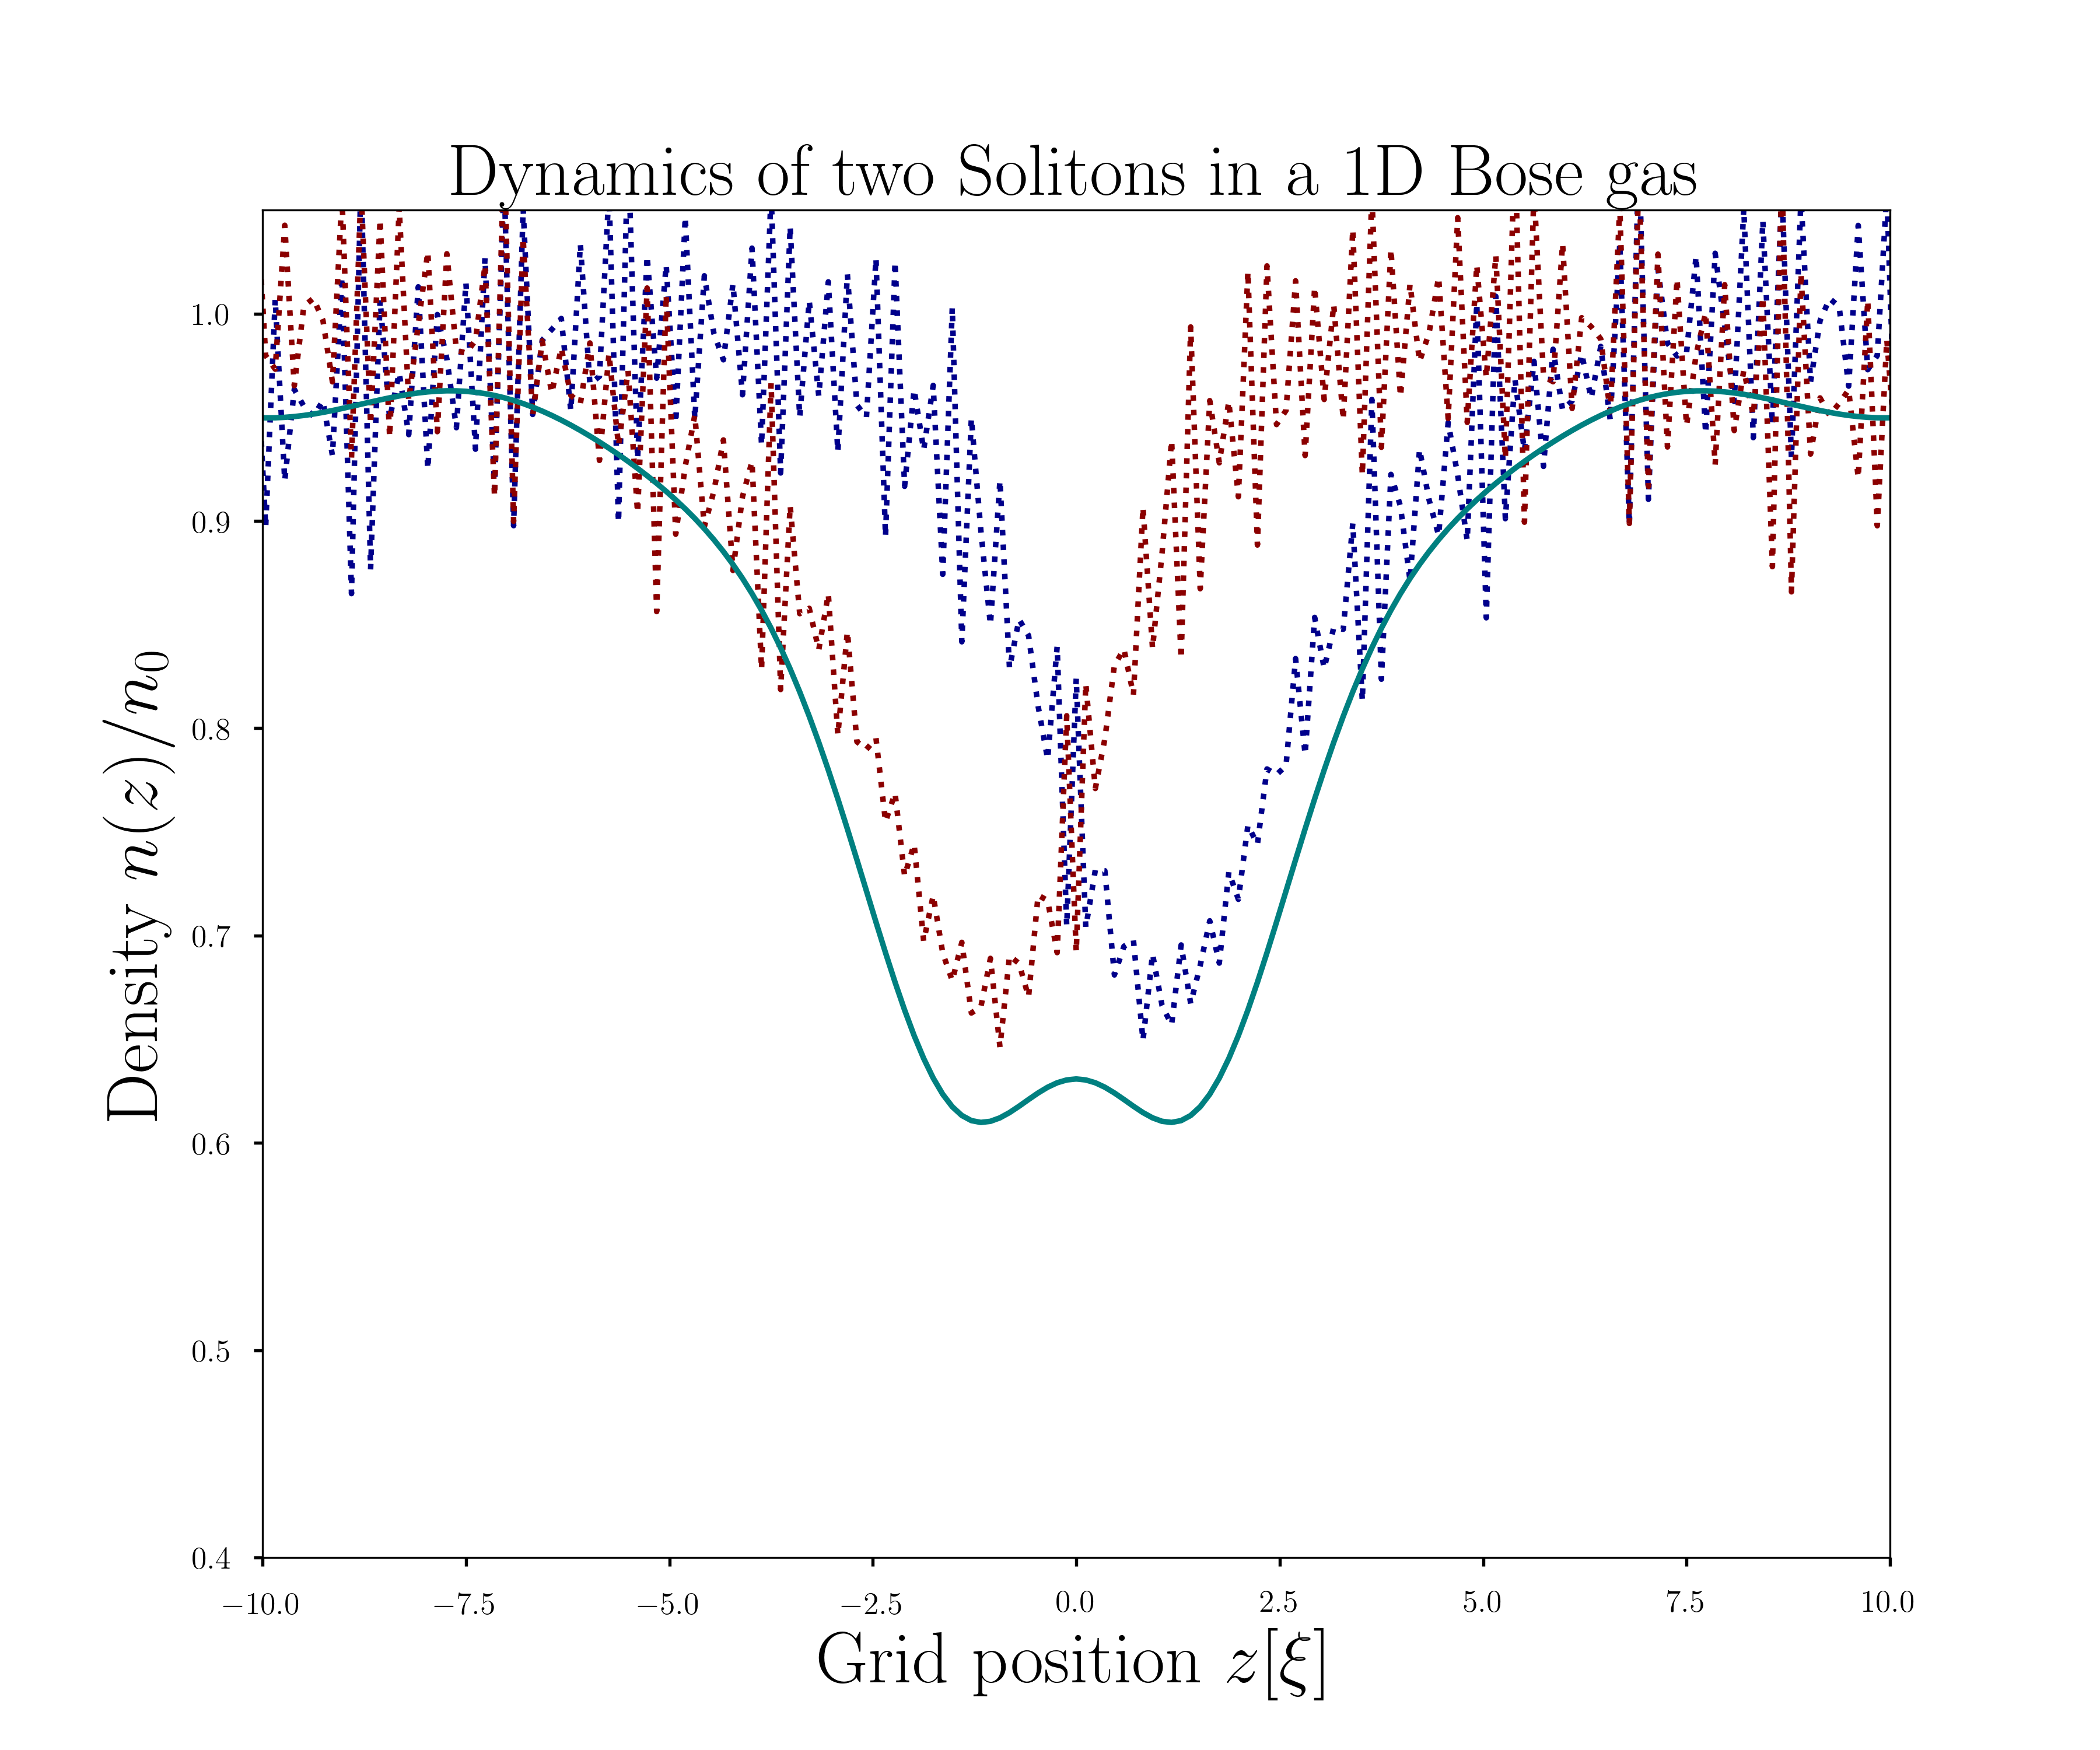
\includegraphics[width= \textwidth]{figures/two_grey_3_5_600}
 	\subcaption{After $N_{\text{steps}} = 600$.}
 \end{subfigure}
 \begin{subfigure}{0.42\textwidth} 
 	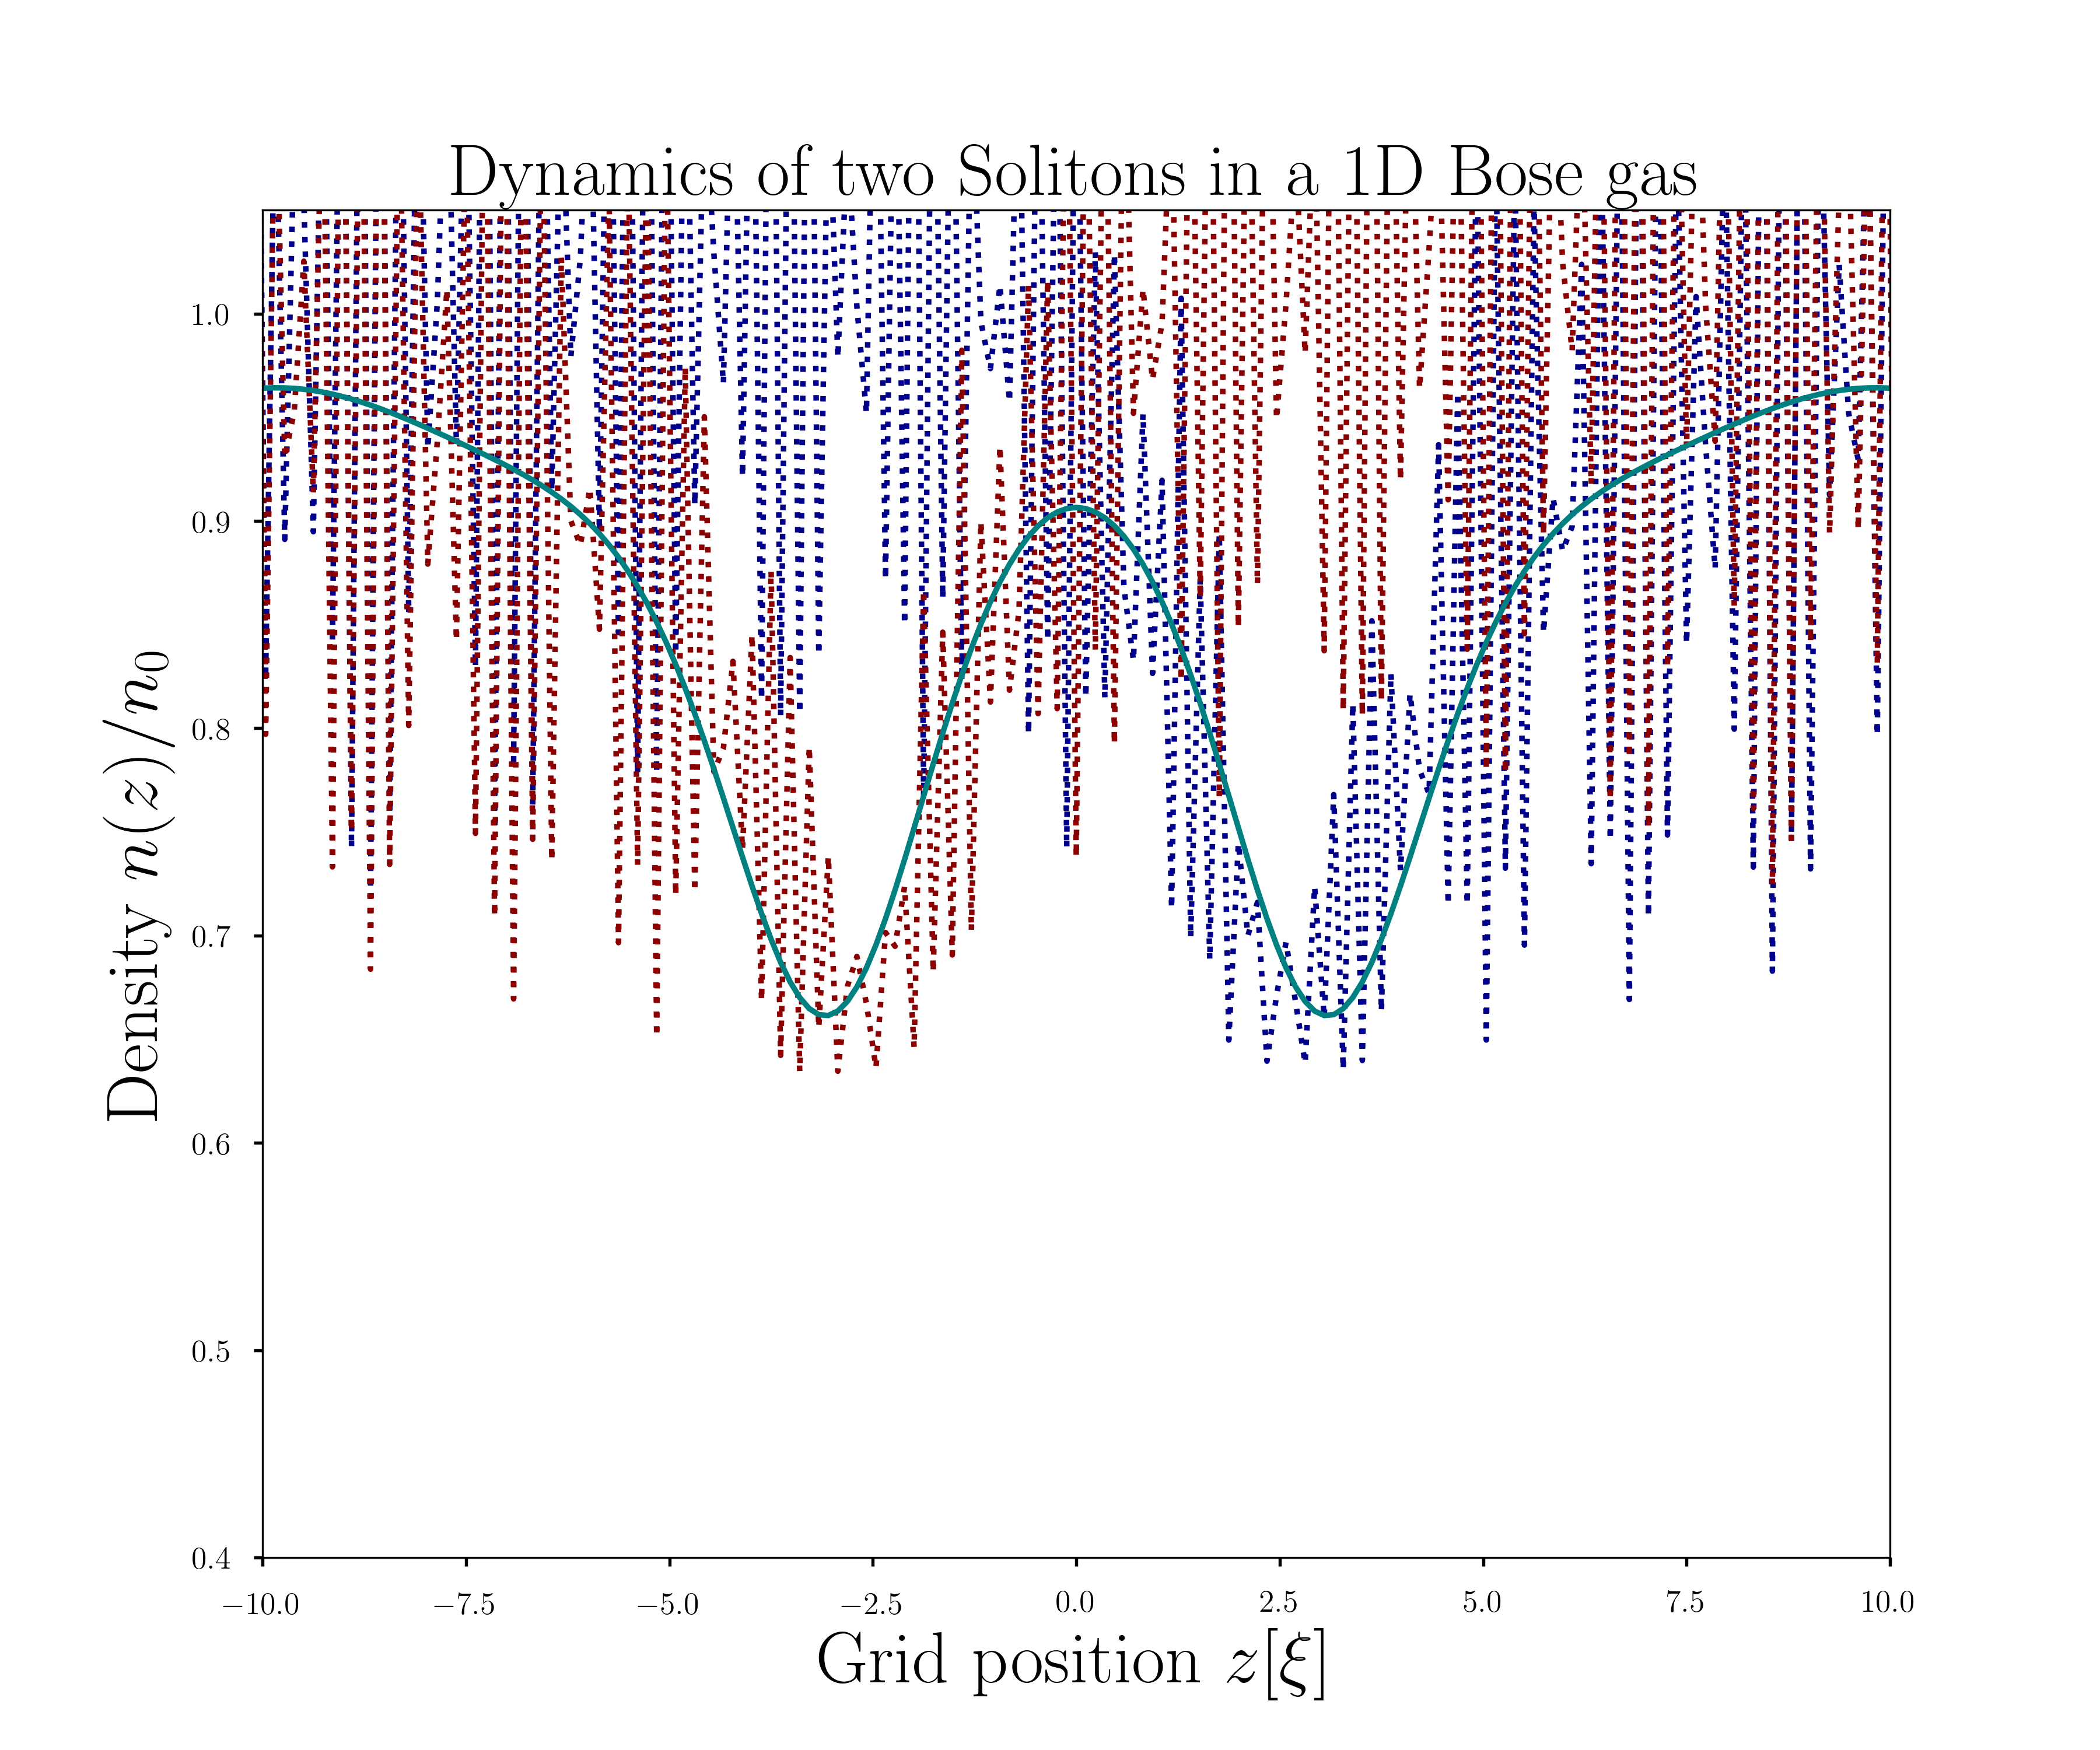
\includegraphics[width= \textwidth]{figures/two_grey_3_5_800}
 	\subcaption{After $N_{\text{steps}} = 800$.}
 \end{subfigure}

 \caption{Dynamics of two grey solitons. The green line shows the superposition of both curves. It seems that the disturbing oscillations cancel each other out.}	
 \end{figure}